\documentclass{article}
\usepackage[utf8]{inputenc}
\usepackage{blindtext}
\usepackage{geometry}
 \geometry{
 a4paper,
 total={170mm,257mm},
 left=25mm,
 right=25mm,
 top=25mm,
 bottom=25mm
 }
\usepackage{url}
 
\usepackage{tikz}
\usetikzlibrary{automata,positioning}

\newcommand{\myset}[1]{\{ #1 \}}
\newcommand{\myor}{\vee}
\newcommand{\myand}{\land}
\newcommand{\setcomplement}[1]{\overline{#1}}
\newcommand{\Alphabet}{\Sigma}
\newcommand{\emptystring}{\epsilon}
\newcommand{\eclose}{\textsc{EClose}}




\newcommand{\mb}[1]{\mathbb{#1}}
\newcommand{\mc}[1]{\mathcal{#1}}
\newcommand{\mt}[1]{\mbox{\tt #1}}
\newcommand{\eq}{\stackrel{.}{=}}
\newcommand{\unify}{\mbox{\tt unify}}
\newcommand{\intt}{\mbox{\tt int}}
\newcommand{\set}[1] {\{ #1  \}}
\newcommand{\sem}[1]{[\![\; #1\; ]\!]}

\newcommand{\lfp}{{\it lfp}}

\newcommand{\mba}{\mathbb{A}}
\newcommand{\mbb}{\mathbb{B}}
\newcommand{\mbc}{\mathbb{C}}
\newcommand{\mbd}{\mathbb{D}}
\newcommand{\mbe}{\mathbb{E}}
\newcommand{\mbf}{\mathbb{F}}
\newcommand{\mbg}{\mathbb{G}}
\newcommand{\mbh}{\mathbb{H}}
\newcommand{\mbi}{\mathbb{I}}
\newcommand{\mbj}{\mathbb{J}}
\newcommand{\mbk}{\mathbb{K}}
\newcommand{\mbl}{\mathbb{L}}
\newcommand{\mbm}{\mathbb{M}}
\newcommand{\mbn}{\mathbb{N}}
\newcommand{\mbo}{\mathbb{O}}
\newcommand{\mbp}{\mathbb{P}}
\newcommand{\mbq}{\mathbb{Q}}
\newcommand{\mbr}{\mathbb{R}}
\newcommand{\mbs}{\mathbb{S}}
\newcommand{\mbt}{\mathbb{T}}
\newcommand{\mbu}{\mathbb{U}}
\newcommand{\mbv}{\mathbb{V}}
\newcommand{\mbw}{\mathbb{W}}
\newcommand{\mbx}{\mathbb{X}}
\newcommand{\mby}{\mathbb{Y}}
\newcommand{\mbz}{\mathbb{Z}}


\newcommand{\power}[1]{\mathcal{P}(#1)}

\newcommand{\domino}[2]{\big[\frac{#1}{#2}\big]}


% %%%% Theorem related macros %%%%
% \newtheorem{solution}{{\bf Solution}}
%\newtheorem{theorem}{{\bf Theorem}}

% \newtheorem{thesis}{{\bf Thesis}}
% \newtheorem{proposition}{{\bf Proposition}}
% \newtheorem{corollary}{{\bf Corollary}}
% \newtheorem{fact}{{\bf Fact}}
% \newtheorem{lemma}{{\bf Lemma}}
% \newtheorem{axiom}{{\bf Axiom}}
% \newtheorem{problem}{{\bf Problem}}
% \newtheorem{conjecture}[theorem]{{\bf Conjecture}}
% \newtheorem{heuristics}[theorem]{{\bf Heuristics}}
% \newtheorem{definition}{{\bf Definition}}
% \newtheorem{example}{{\bf Example}}
% \newtheorem{exercise}{{\bf Exercise}}
% \newtheorem{project}{{\bf Project}}
% \newtheorem{viewpoint}{{\bf ViewPoint}}
% \newtheorem{property}{{\bf Property}}
% \newtheorem{homework}{{\bf Homework}}
% \newtheorem{ghomework}{{\bf Homework$\star$}}
% \newtheorem{challenge}{{\bf Challenge}}
% \newtheorem{side}{{\bf Side Note}}
% \newtheorem{quiz}{{\bf Check}}

% \newcommand{\Quiz}[1]{\begin{quiz}{\rm #1}\end{quiz}}
% \newcommand{\Side}[1]{\begin{side}{\rm #1}\end{side}}
% \newcommand{\Challenge}[1]{\begin{challenge}{\rm #1}\end{challenge}}
% \newcommand{\Exercise}[1]{\begin{exercise}{\rm #1}\end{exercise}}
% \newcommand{\Project}[1]{\begin{project}{\rm #1}\end{project}}
% \newcommand{\Problem}[1]{\begin{problem}{\rm #1}\end{problem}}
% \newcommand{\Homework}[1]{\begin{exercise}{\rm #1}\end{exercise}}
% \newcommand{\GHomework}[1]{\begin{exercise}{\rm #1}\end{exercise}}
% \newcommand{\Definition}[1]{\begin{definition} #1\end{definition}}
% \newcommand{\Deffinition}[2]{\begin{definition}[#1] #2\end{definition}}
% \newcommand{\NDefinition}[2]{\begin{definition}[#1] #2\end{definition}}
% \newcommand{\Solution}[1]{\begin{solution} #1\end{solution}}
% \newcommand{\Theorem}[1]{\begin{theorem} #1 \end{theorem}}
% \newcommand{\NTheorem}[2]{\begin{theorem}[#1] #2\end{theorem}}
% \newcommand{\Thesis}[1]{\begin{thesis} #1 \end{thesis}}
% \newcommand{\Fact}[1]{\begin{fact} #1 \end{fact}}
% \newcommand{\Property}[1]{\begin{property} #1 \end{property}}
% \newcommand{\Proposition}[1]{\begin{proposition} #1 \end{proposition}}
% \newcommand{\NProposition}[2]{\begin{proposition}[#1] #2 \end{proposition}}
% \newcommand{\Corollary}[1]{\begin{corollary} #1 \end{corollary}}
% \newcommand{\NCorollary}[2]{\begin{corollary}[#1] #2 \end{corollary}}
% \newcommand{\Example}[1]{\begin{example}{\rm #1}$\Box$\end{example}}
% \newcommand{\Axiom}[1]{\begin{axiom}{\rm #1}\end{axiom}}
% \newcommand{\Conjecture}[1]{\begin{conjecture} #1 \end{conjecture}}
% \newcommand{\Heuristic}[1]{\begin{heuristics} #1 \end{heuristics}}
% \newcommand{\Lemma}[1]{\begin{lemma} #1 \end{lemma}}
%\newcommand{\Proof}[1]{{\it Proof}. #1 \hspace*{\fill}$\Box$\par}
% \newcommand{\Proof}[1]{{\it Proof}. #1 $\Box$\par}
% \newcommand{\Sketch}[1]{{\it Proof Sketch}. #1 $\Box$\par}
% \newcommand{\Viewpoint}[1]{\begin{viewpoint} #1 \end{viewpoint}}




\title{CSE332 Theory of Computation \\ Homework 1}
\author{Student: Azizbek Umidjonov 20202043}
\date{Due: Tuesday, October 11, 2022 at 11:59pm on Blackboard}

\begin{document}

\maketitle

\section*{Solutions} 

\noindent \textbf{Problem 1}
\begin{itemize}
\item \textbf{Base case:} Let u be an arbitrary string of length 0. u = {$\epsilon$} since there is only one such string. Then $(uv)^{R} = (\epsilon v)^R = v^R = v^R \epsilon = v^R \epsilon^R =  v^{R}u^{R}$
\item \textbf{Induction hypothesis:} {$\forall n \ge 0$}, for any string u of length n:
For all strings {$v \in \Alphabet^{+}, (uv)^R = u^R v^R$}. No assumption about v, hence statement holds for all {$v \in \Alphabet^{+}$}
\end{itemize}
    
\noindent \textbf{Problem 2}
    \begin{itemize}
        \item DFA:
        \begin{center}
            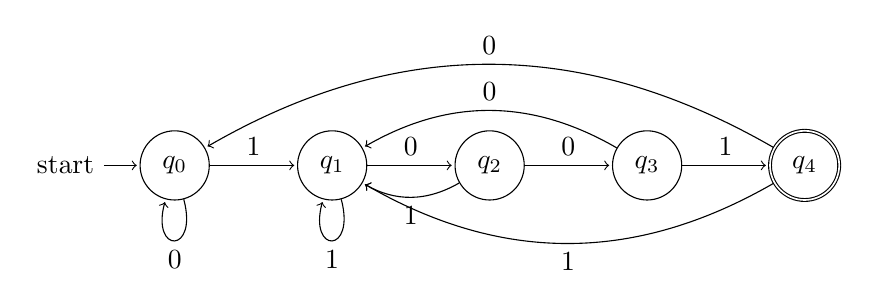
\begin{tikzpicture}[shorten >=1pt,node distance=2cm,on grid,auto] 
                \node[state,initial] (q_0)   {$q_0$}; 
                \node[state] (q_1) [right=of q_0] {$q_1$}; 
                \node[state] (q_2) [right=of q_1] {$q_2$};
                \node[state] (q_3) [right=of q_2] {$q_3$};
                \node[state,accepting] (q_4) [right=of q_3] {$q_4$}; 
                \path[->]
                (q_0) edge [loop below] node {$0$} ()
                (q_0) edge node {$1$} (q_1)
                (q_1) edge node {$0$} (q_2)
                (q_1) edge [loop below] node {$1$} ()
                (q_2) edge [above] node {$0$} (q_3)
                (q_2) edge [bend left, below] node {$1$} (q_1)
                (q_3) edge [bend right, above] node {$0$} (q_1)
                (q_3) edge node {$1$} (q_4)
                (q_4) edge [bend right, above] node {$0$} (q_0)
                (q_4) edge [bend left, below] node {$1$} (q_1);
            \end{tikzpicture}
        \end{center}
        \item NFA
        \begin{center}
            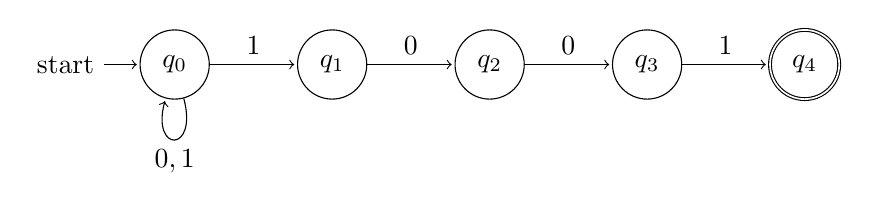
\begin{tikzpicture}[shorten >=1pt,node distance=2cm,on grid,auto] 
                \node[state,initial] (q_0)   {$q_0$}; 
                \node[state] (q_1) [right=of q_0] {$q_1$}; 
                \node[state] (q_2) [right=of q_1] {$q_2$};
                \node[state] (q_3) [right=of q_2] {$q_3$};
                \node[state,accepting] (q_4) [right=of q_3] {$q_4$}; 
                \path[->]
                (q_0) edge [loop below] node {$0,1$} ()
                (q_0) edge node {$1$} (q_1)
                (q_1) edge node {$0$} (q_2)
                (q_2) edge node {$0$} (q_3)
                (q_3) edge node {$1$} (q_4);
            \end{tikzpicture}
        \end{center}
    \end{itemize}
    
\noindent \textbf{Problem 3} 
    \begin{center}
        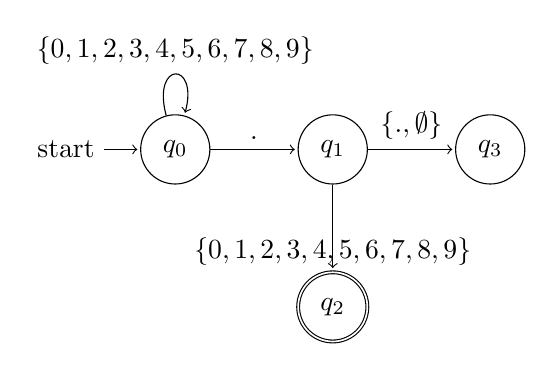
\begin{tikzpicture}[shorten >=1pt,node distance=2cm,on grid,auto] 
            \node[state,initial] (q_0)   {$q_0$}; 
            \node[state] (q_1) [right=of q_0] {$q_1$}; 
            \node[state,accepting] (q_2) [below=of q_1] {$q_2$};
            \node[state] (q_3) [right=of q_1] {$q_3$};
            \path[->]
            (q_0) edge [loop above] node {$\{0,1,2,3,4,5,6,7,8,9\}$} ()
            (q_0) edge node {$.$} (q_1)
            (q_1) edge [below] node {$\{0,1,2,3,4,5,6,7,8,9\}$} (q_2)
            (q_1) edge node {$\{., \emptyset\}$} (q_3);
        \end{tikzpicture}
    \end{center}
    

\noindent \newline \textbf{Problem 4}
\begin{itemize}
    \item NFA
        \begin{center}
            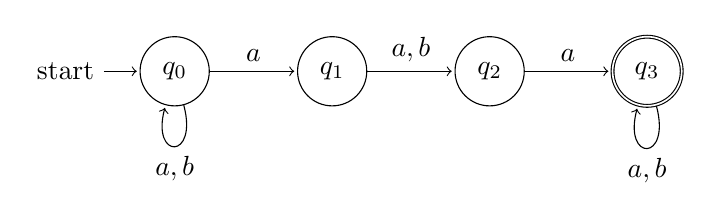
\begin{tikzpicture}[shorten >=1pt,node distance=2cm,on grid,auto] 
                \node[state,initial] (q_0)   {$q_0$}; 
                \node[state] (q_1) [right=of q_0] {$q_1$}; 
                \node[state] (q_2) [right=of q_1] {$q_2$};
                \node[state,accepting] (q_3) [right=of q_2] {$q_3$}; 
                \path[->]
                (q_0) edge node {$a$} (q_1)
                (q_1) edge node {$a,b$} (q_2)
                (q_2) edge node {$a$} (q_3)
                (q_0) edge [loop below] node {$a,b$} ()
                (q_3) edge [loop below] node {$a,b$} ();
            \end{tikzpicture}
        \end{center}
    \item DFA 
        \begin{center}
            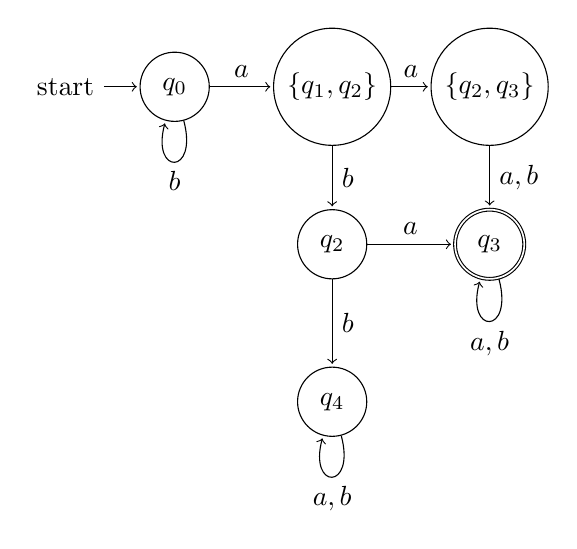
\begin{tikzpicture}[shorten >=1pt,node distance=2cm,on grid,auto] 
                \node[state,initial] (q_0)   {$q_0$}; 
                \node[state] (q12) [right=of q_0] {$\{q_1, q_2\}$};
                \node[state] (q23) [right=of q12] {$\{q_2, q_3\}$};
                \node[state] (q_2) [below=of q12] {$q_2$};
                \node[state,accepting] (q_3) [below=of q23] {$q_3$}; 
                \node[state] (q_4) [below=of q_2] {$q_4$};
        
                \path[->]
                (q_0) edge [loop below] node {$b$} ()
                (q_0) edge node {$a$} (q12)
                (q12) edge node {$a$} (q23)
                (q12) edge node {$b$} (q_2)
                (q23) edge node {$a,b$} (q_3)
                (q_2) edge node {$a$} (q_3)
                (q_2) edge node {$b$} (q_4)
                (q_3) edge [loop below] node {$a,b$} ()
                (q_4) edge [loop below] node {$a,b$} ();
            \end{tikzpicture}
        \end{center}
\end{itemize}



\noindent \textbf{Problem 5} (10pts) Design an $\epsilon$-NFA that accepts the following language:
\begin{center}
    $L = \{a^{m}b^{n}c^{o}\,|\,m,n,o \geq 0\}$
\end{center}

\begin{center}
\textbf{1st version:}
\end{center}
\begin{center}
            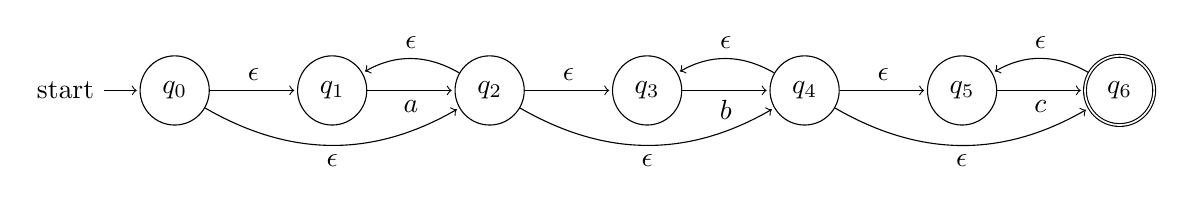
\begin{tikzpicture}[shorten >=1pt,node distance=2cm,on grid,auto] 
                \node[state,initial] (q_0)   {$q_0$}; 
                \node[state] (q_1) [right=of q_0] {$q_1$};
                \node[state] (q_2) [right=of q_1] {$q_2$};
                \node[state] (q_3) [right=of q_2] {$q_3$};
                \node[state] (q_4) [right=of q_3] {$q_4$};
                \node[state] (q_5) [right=of q_4] {$q_5$};
                \node[state, accepting] (q_6) [right=of q_5] {$q_6$};
        
                \path[->]
                (q_0) edge node {$\epsilon$} (q_1)
                (q_0) edge [bend right, below] node {$\epsilon$} (q_2)
                (q_1) edge [below] node {$a$} (q_2)
                (q_2) edge node {$\epsilon$} (q_3)
                (q_2) edge [bend right, above] node {$\epsilon$} (q_1)
                (q_2) edge [bend right, below] node {$\epsilon$} (q_4)
                (q_3) edge [below] node {$b$} (q_4)
                (q_4) edge node {$\epsilon$} (q_5)
                (q_4) edge [bend right, above] node {$\epsilon$} (q_3)
                (q_4) edge [bend right, below] node {$\epsilon$} (q_6)
                (q_5) edge [below] node {$c$} (q_6)
                (q_6) edge [bend right, above] node {$\epsilon$} (q_5);
                
            \end{tikzpicture}
        \end{center}
\begin{center}
\textbf{2nd version:}
\end{center}
\begin{center}
            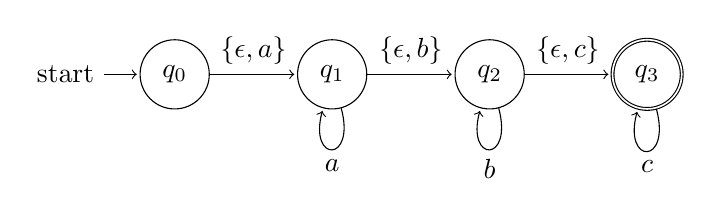
\begin{tikzpicture}[shorten >=1pt,node distance=2cm,on grid,auto] 
                \node[state,initial] (q_0)   {$q_0$}; 
                \node[state] (q_1) [right=of q_0] {$q_1$};
                \node[state] (q_2) [right=of q_1] {$q_2$};
                \node[state, accepting] (q_3) [right=of q_2] {$q_3$};
                \path[->]
                (q_0) edge node {$\{\epsilon, a\}$} (q_1)
                (q_1) edge node {$\{\epsilon, b\}$} (q_2)             
                (q_2) edge node {$\{\epsilon, c\}$} (q_3)
                (q_1) edge [loop below] node {$a$} ()
                (q_2) edge [loop below] node {$b$} ()
                (q_3) edge [loop below] node {$c$} ();
            \end{tikzpicture}
        \end{center}

\noindent \textbf{Problem 6} (20pts) Consider the following transition table of an $\epsilon$-NFA:
    \begin{center}
    \small
        \begin{tabular}{r||c|c|c|c}
        & $\epsilon$ & $a$ & $b$ & $c$\\ \hline\hline
        $p$ & $\emptyset$ & $\{p\}$ & $\{q\}$ & $\{r\}$\\ 
        $q$ & $\{p\}$ & $\{q\}$ & $\{r\}$ & $\emptyset$\\ 
        $r$ & $\{q\}$ & $\{r\}$ & $\emptyset$ & $\{p\}$\\ 
        \end{tabular}
    \end{center}
    where $p$ is the initial state and $r$ is the final state.
    \begin{enumerate}
        \item (10pts) Compute the $\epsilon$-closure(EClosure) of each state.
        \item (10pts) Convert the automaton to a DFA.
    \end{enumerate}
    
\noindent \textbf{Problem 7} (15pts, 5pts each) Find regular expressions for the following languages.
\begin{enumerate}
    \item $L = \myset{\omega \in \myset{a,b,c}^* \mid \omega \mbox{ has no more than three $a$'s}}$
    \item $L = \myset{\omega \in \myset{0,1}^* \mid \omega \mbox{ begins and ends with 0 and contains at least one 1}}$
    \item $L = \myset{\omega \in \myset{0,1}^* \mid \omega \mbox{ does not contain 111}}$ 
    % \item $S = \myset{2,4,6,\dots} = \myset{x \in \mbn \mid \mbox{$x$ is even}}$
\end{enumerate}

\noindent \textbf{Problem 8} (20pts) Consider a DFA represented by a transition table:
\begin{center}
\small
\begin{tabular}{r|c|c}
& 0 & 1 \\ \hline
$\rightarrow q_1$ & $q_2$ & $q_1$ \\ 
$q_2$ & $q_3$ & $q_1$ \\ 
$*q_3$ & $q_3$ & $q_2$
\end{tabular}
\end{center}
Give all the regular expressions $R^{(0)}_{ij}$,$R^{(1)}_{ij}$,$R^{(2)}_{ij}$. Try to simplify the expressions as much as possible.
Think of state $q_i$ as if it were the state with number $i$.

\noindent \newline \textbf{Problem 9} (10pts) Convert the following regular expressions to finite automata ($\epsilon$-NFA): $ab^*aa+bba^*ab$ \\

\noindent \textbf{Problem 10} (10pts) Find a $\epsilon$-NFA that accepts language $L(ab^*a^*)\cap L(a^*b^*a)$.


\end{document}

